\chapter{Dossier fonctionnel}
\section{Ingénierie des exigences}
\subsection{Approche Top-Down}
\label{sec:top-down}

Pour notre approche Top-Down, nous sommes revenus à la demande initiale du projet : remplacer la souris d'un ordinateur par le mouvement oculaire de l'utilisateur. La fonction principale du système est donc apparue clairement : permettre à l'utilisateur d'interagir avec une interface via ses yeux. 

\begin{figure}[h]
  \centering
  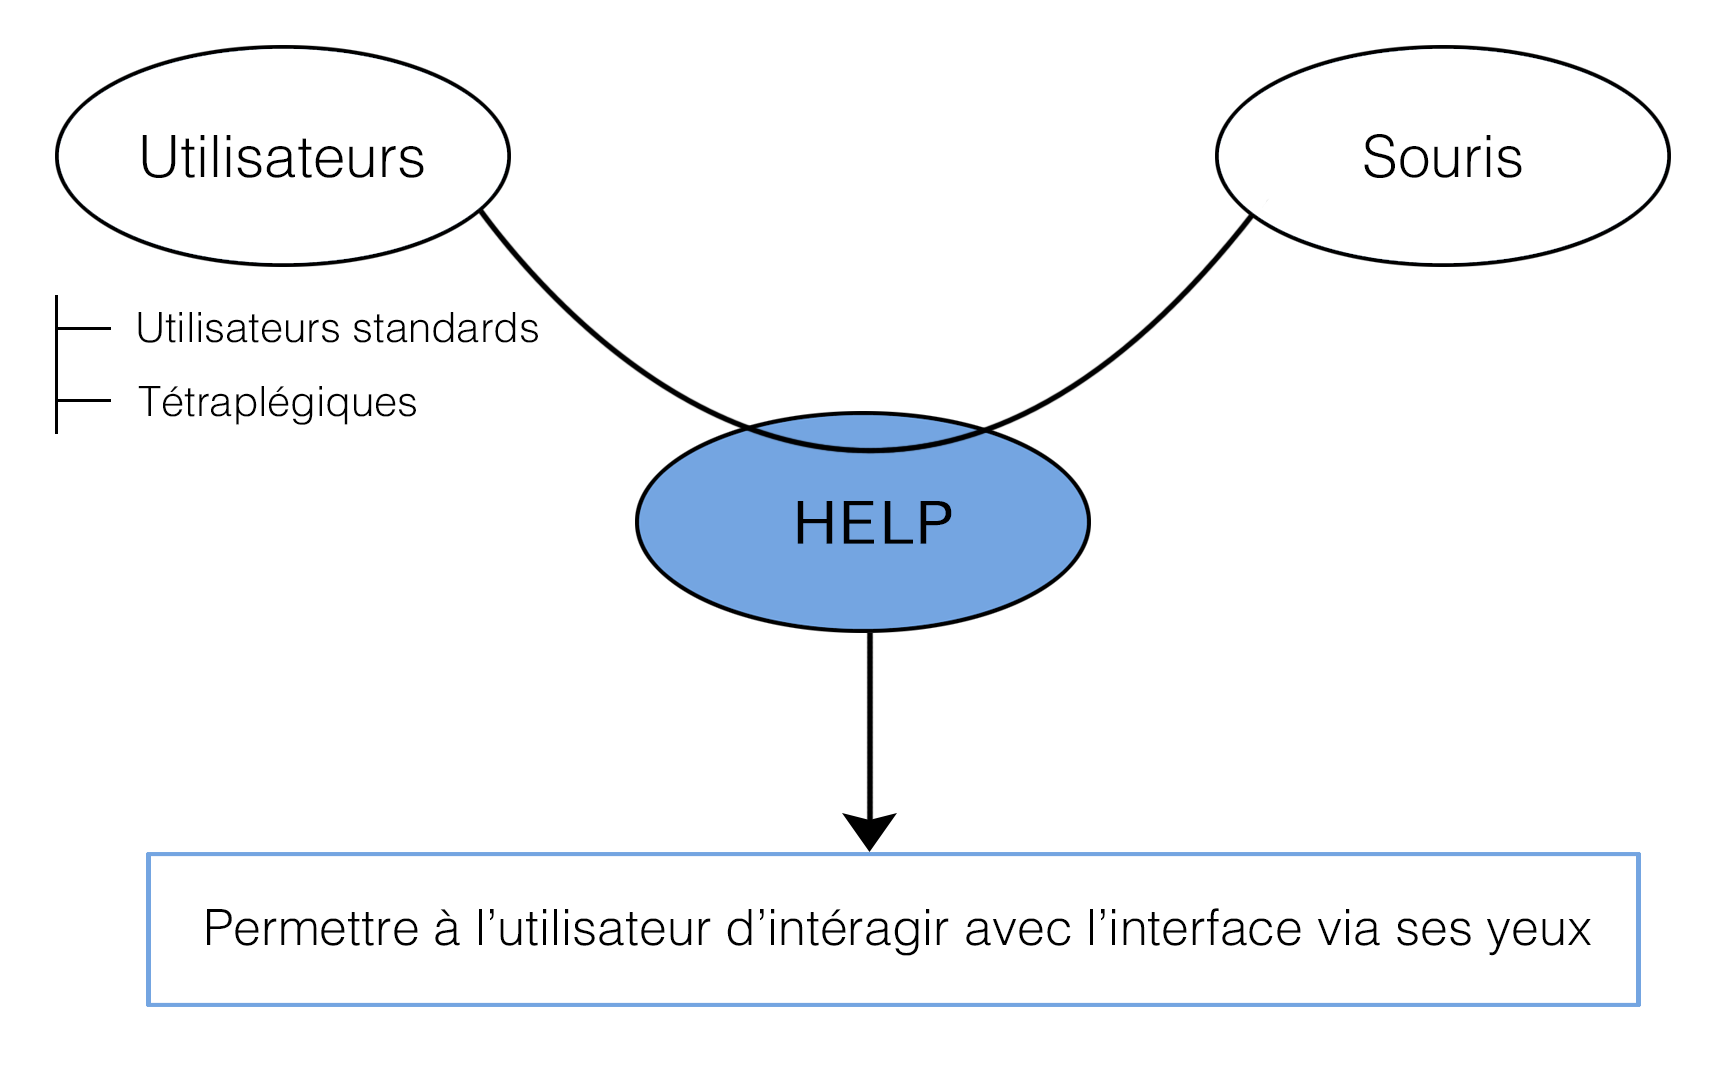
\includegraphics[scale=1]{BeteACornes}
  \caption{Bête à cornes}
  \label{fig:bac}
\end{figure}

Dans la suite du dossier fonctionnel, nous avons supposé que nous utilisions deux caméras. Dans les faits, comme nous l'avons précisé dans les méthodes de réalisation choisies (paragraphe \ref{MethodesChoisies}), nous n'avons pas eu le temps de configurer les deux webcams. Le système a toutefois gardé la même démarche, une caméra réalisant à la fois la détection du visage et du centre des pupilles. 

D'autre part, dans le diagramme pieuvre (figure \ref{fig:pieuvre}), nous avons défini la fonction de contrainte sur la sécurité de l'utilisateur. En effet, ce critère est important, notamment dans le cas d'essais cliniques sur des personnes tétraplégiques. Notre système n'étant pas encore au point, nous n'avons pas eu l'occasion de nous mettre en relation avec de tels utilisateurs. Néanmoins, nous pensons que les autorités règlementaires concernées valideraient les tests. N'utilisant pas d'infrarouge, le système, composé d'un ordinateur et d'une ou deux caméras nous semble fiable. 

\begin{figure}[H]
  \centering
  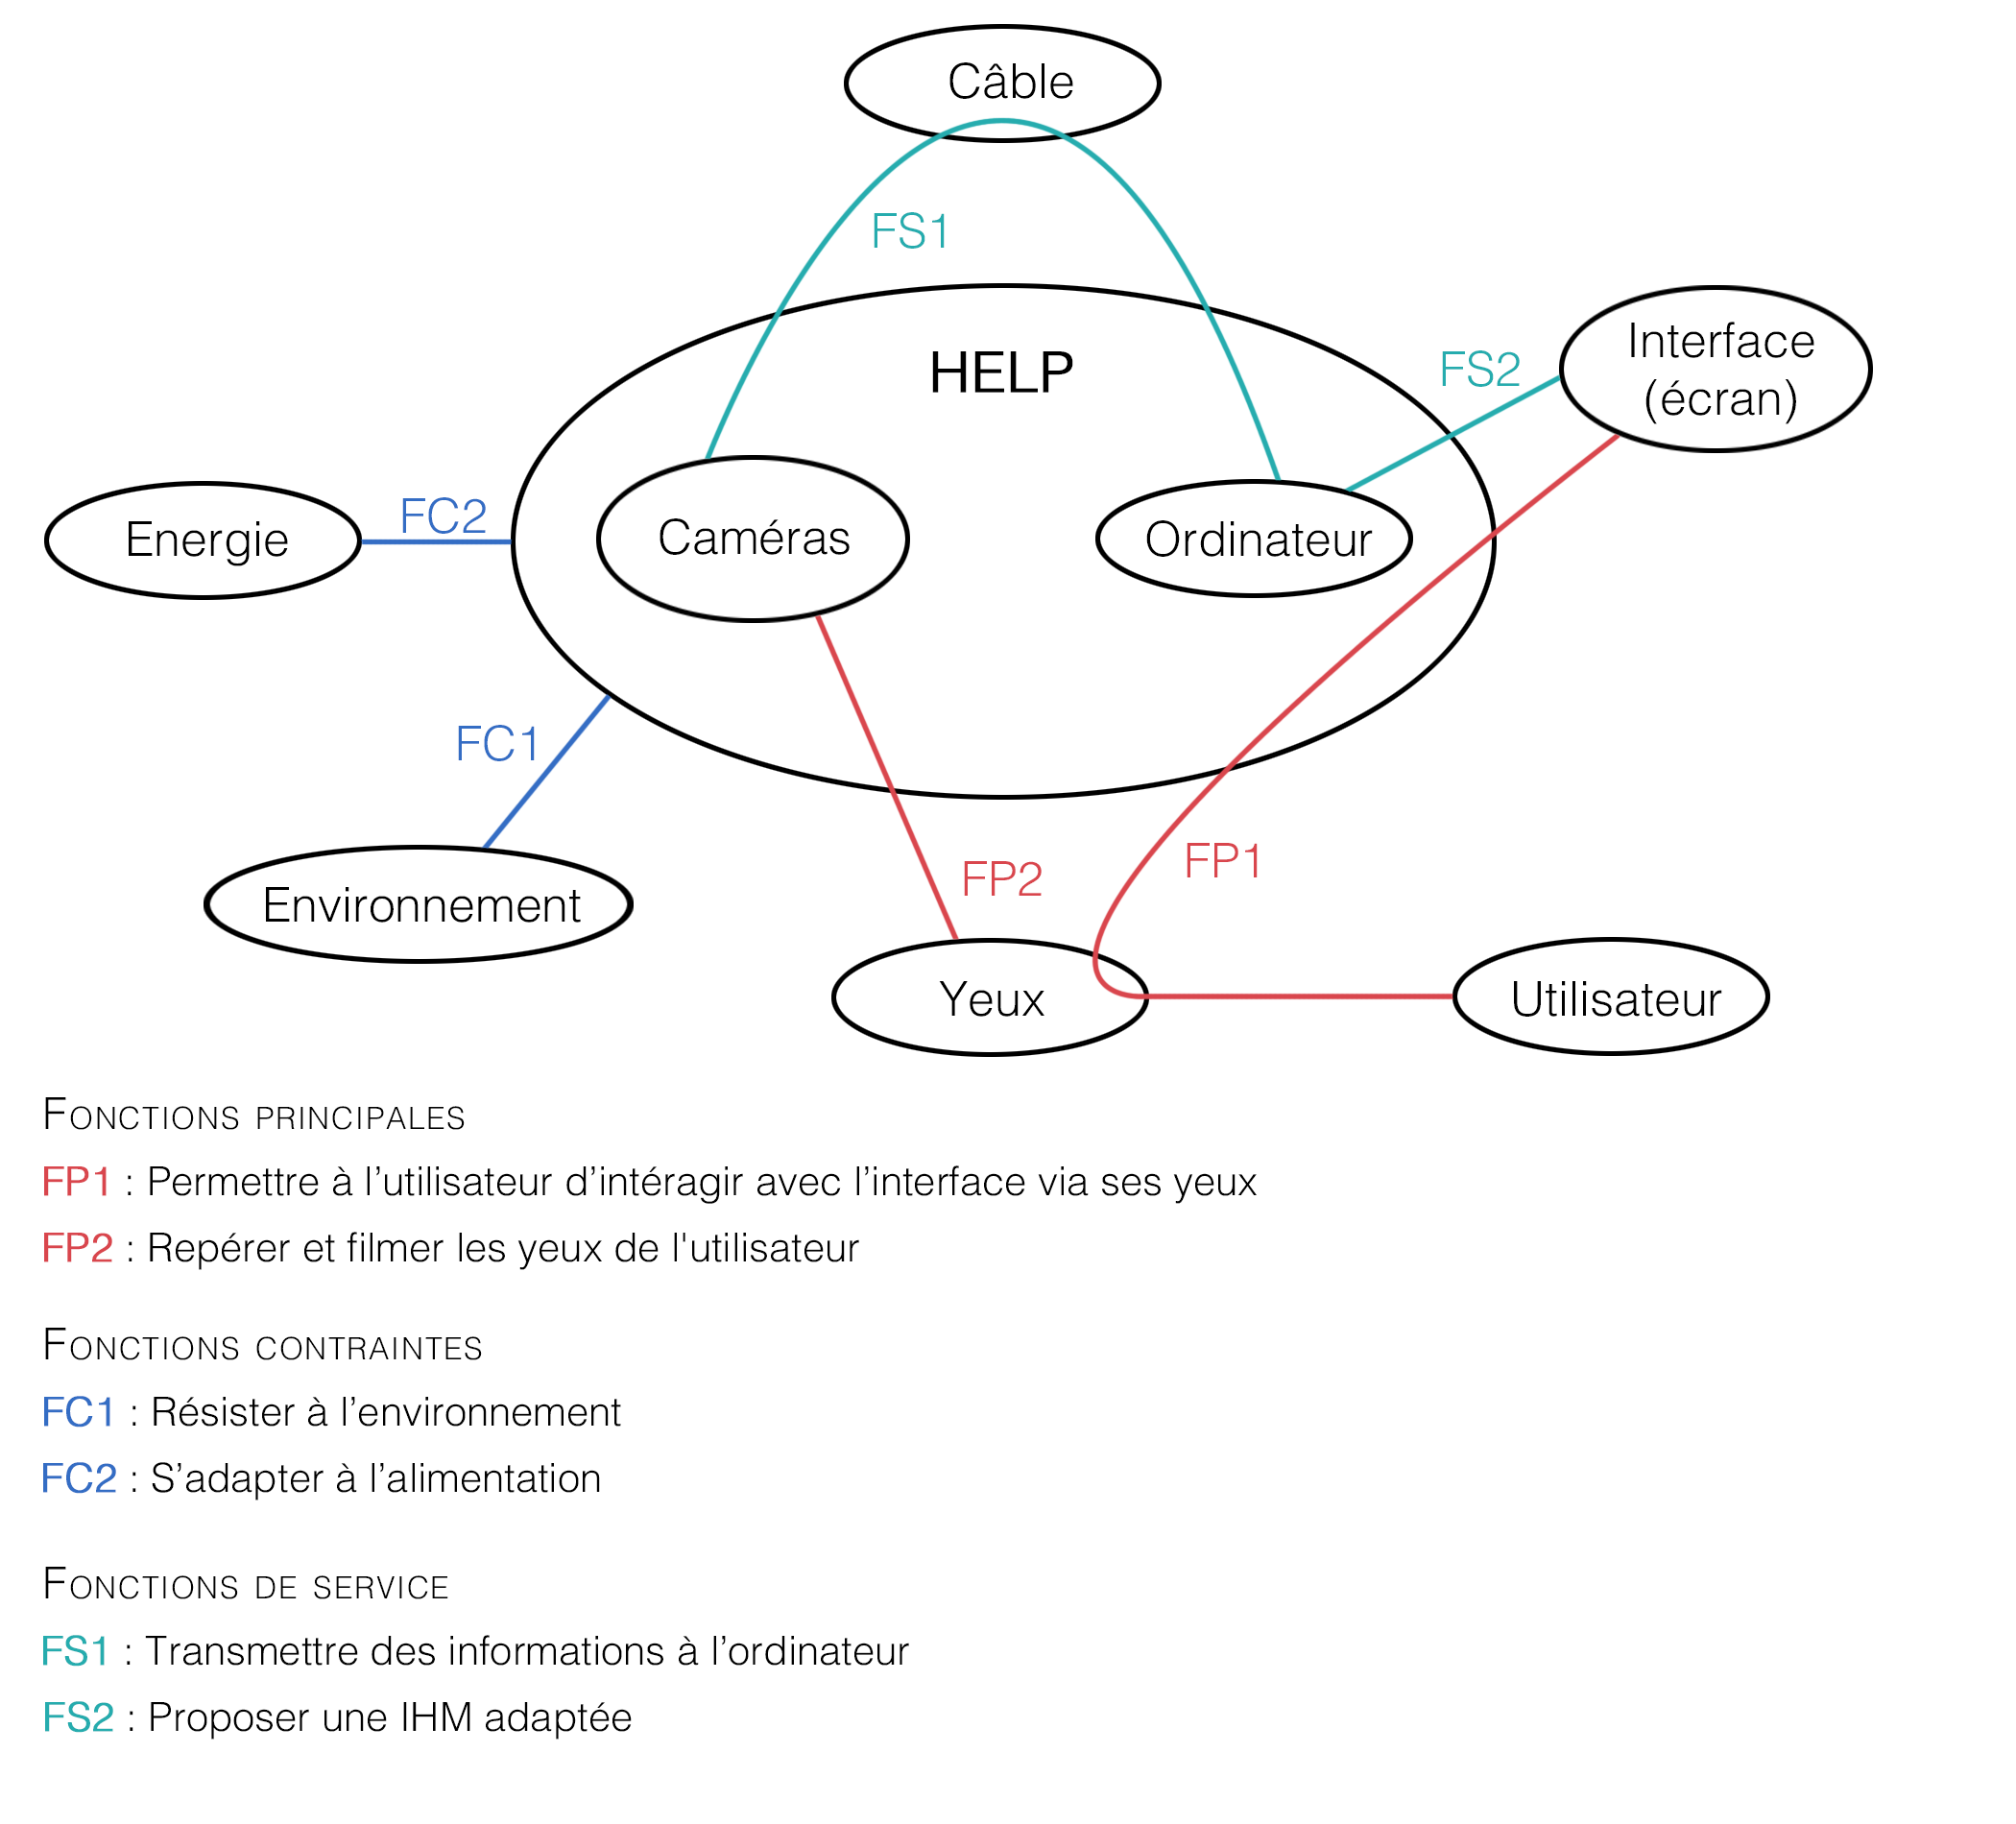
\includegraphics[scale=0.9]{PieuvreV2}
  \caption{Diagramme pieuvre}
  \label{fig:pieuvre}
\end{figure}

\subsection{Approche Bottom-Up}
\definecolor{sable}{RGB}{238,236,225}
Nous avons défini les différentes exigences auxquelles le système devra répondre, indépendamment de nos choix de réalisation technique. Nous les avons alors rassemblées par groupement logique, ce qui nous permettra de définir nos fonctions principales. Les lignes en {\color{sable}{\rule{0.5cm}{0.25cm}}} sont uniquement valables pour la méthode embarquant un système sur l'utilisateur. Elles sont donc à ignorer dans un premier temps puisque nous avons choisi une approche différente. 

\begin{figure}[H]
  \centering
  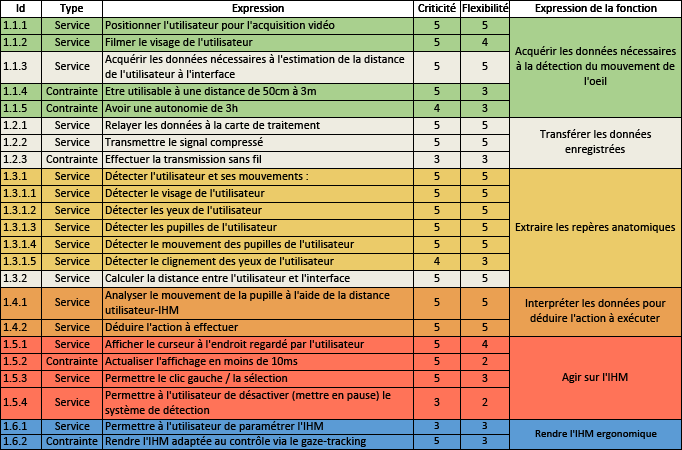
\includegraphics[width=\textwidth]{CahierdesExigencesV4}
  \caption{Cahier des exigences (les critères de criticité et de flexibilité sont sur 5)}
  \label{fig:exigences}
\end{figure}

\subsection{Fonctions principales du système}

Dans le cadre de ce projet, nous cherchons donc à remplacer la souris d'un ordinateur par un système qui suit le mouvement des yeux de l'utilisateur. Pour ce faire, nous avons mis en évidence des groupements logiques d'exigence. Tout d'abord, le système doit acquérir les données nécessaires à la détection du mouvement de l'œil. Ces données devront alors être traitées par l'ordinateur. Ce dernier doit alors interpréter ces données pour en déduire l'action à exécuter. De ces nouvelles informations, l'ordinateur doit pouvoir effectuer l'action que l'utilisateur veut effectuer sur l'IHM, la mettre en place, et montrer que ces modifications ont été exécutées. 

\begin{itemize}[label=\textbullet,font=\color{black}]
\item FP1 : Acquérir les données nécessaire à la détection du mouvement de l'œil 
\item\colorbox{sable}{FP2 : Transférer les données enregistrées}
\item FP3 : Extraire les repères anatomiques
\item FP4 : Interpréter les données pour déduire l'action à exécuter 
\item FP5 : Agir sur l'IHM
\item FP6 : Rendre l'IHM ergonomique
\end{itemize}

\section{Spécification fonctionnelle  3 axes}

\subsection{Raffinement FAST}

\begin{figure}[H]
  \centering
  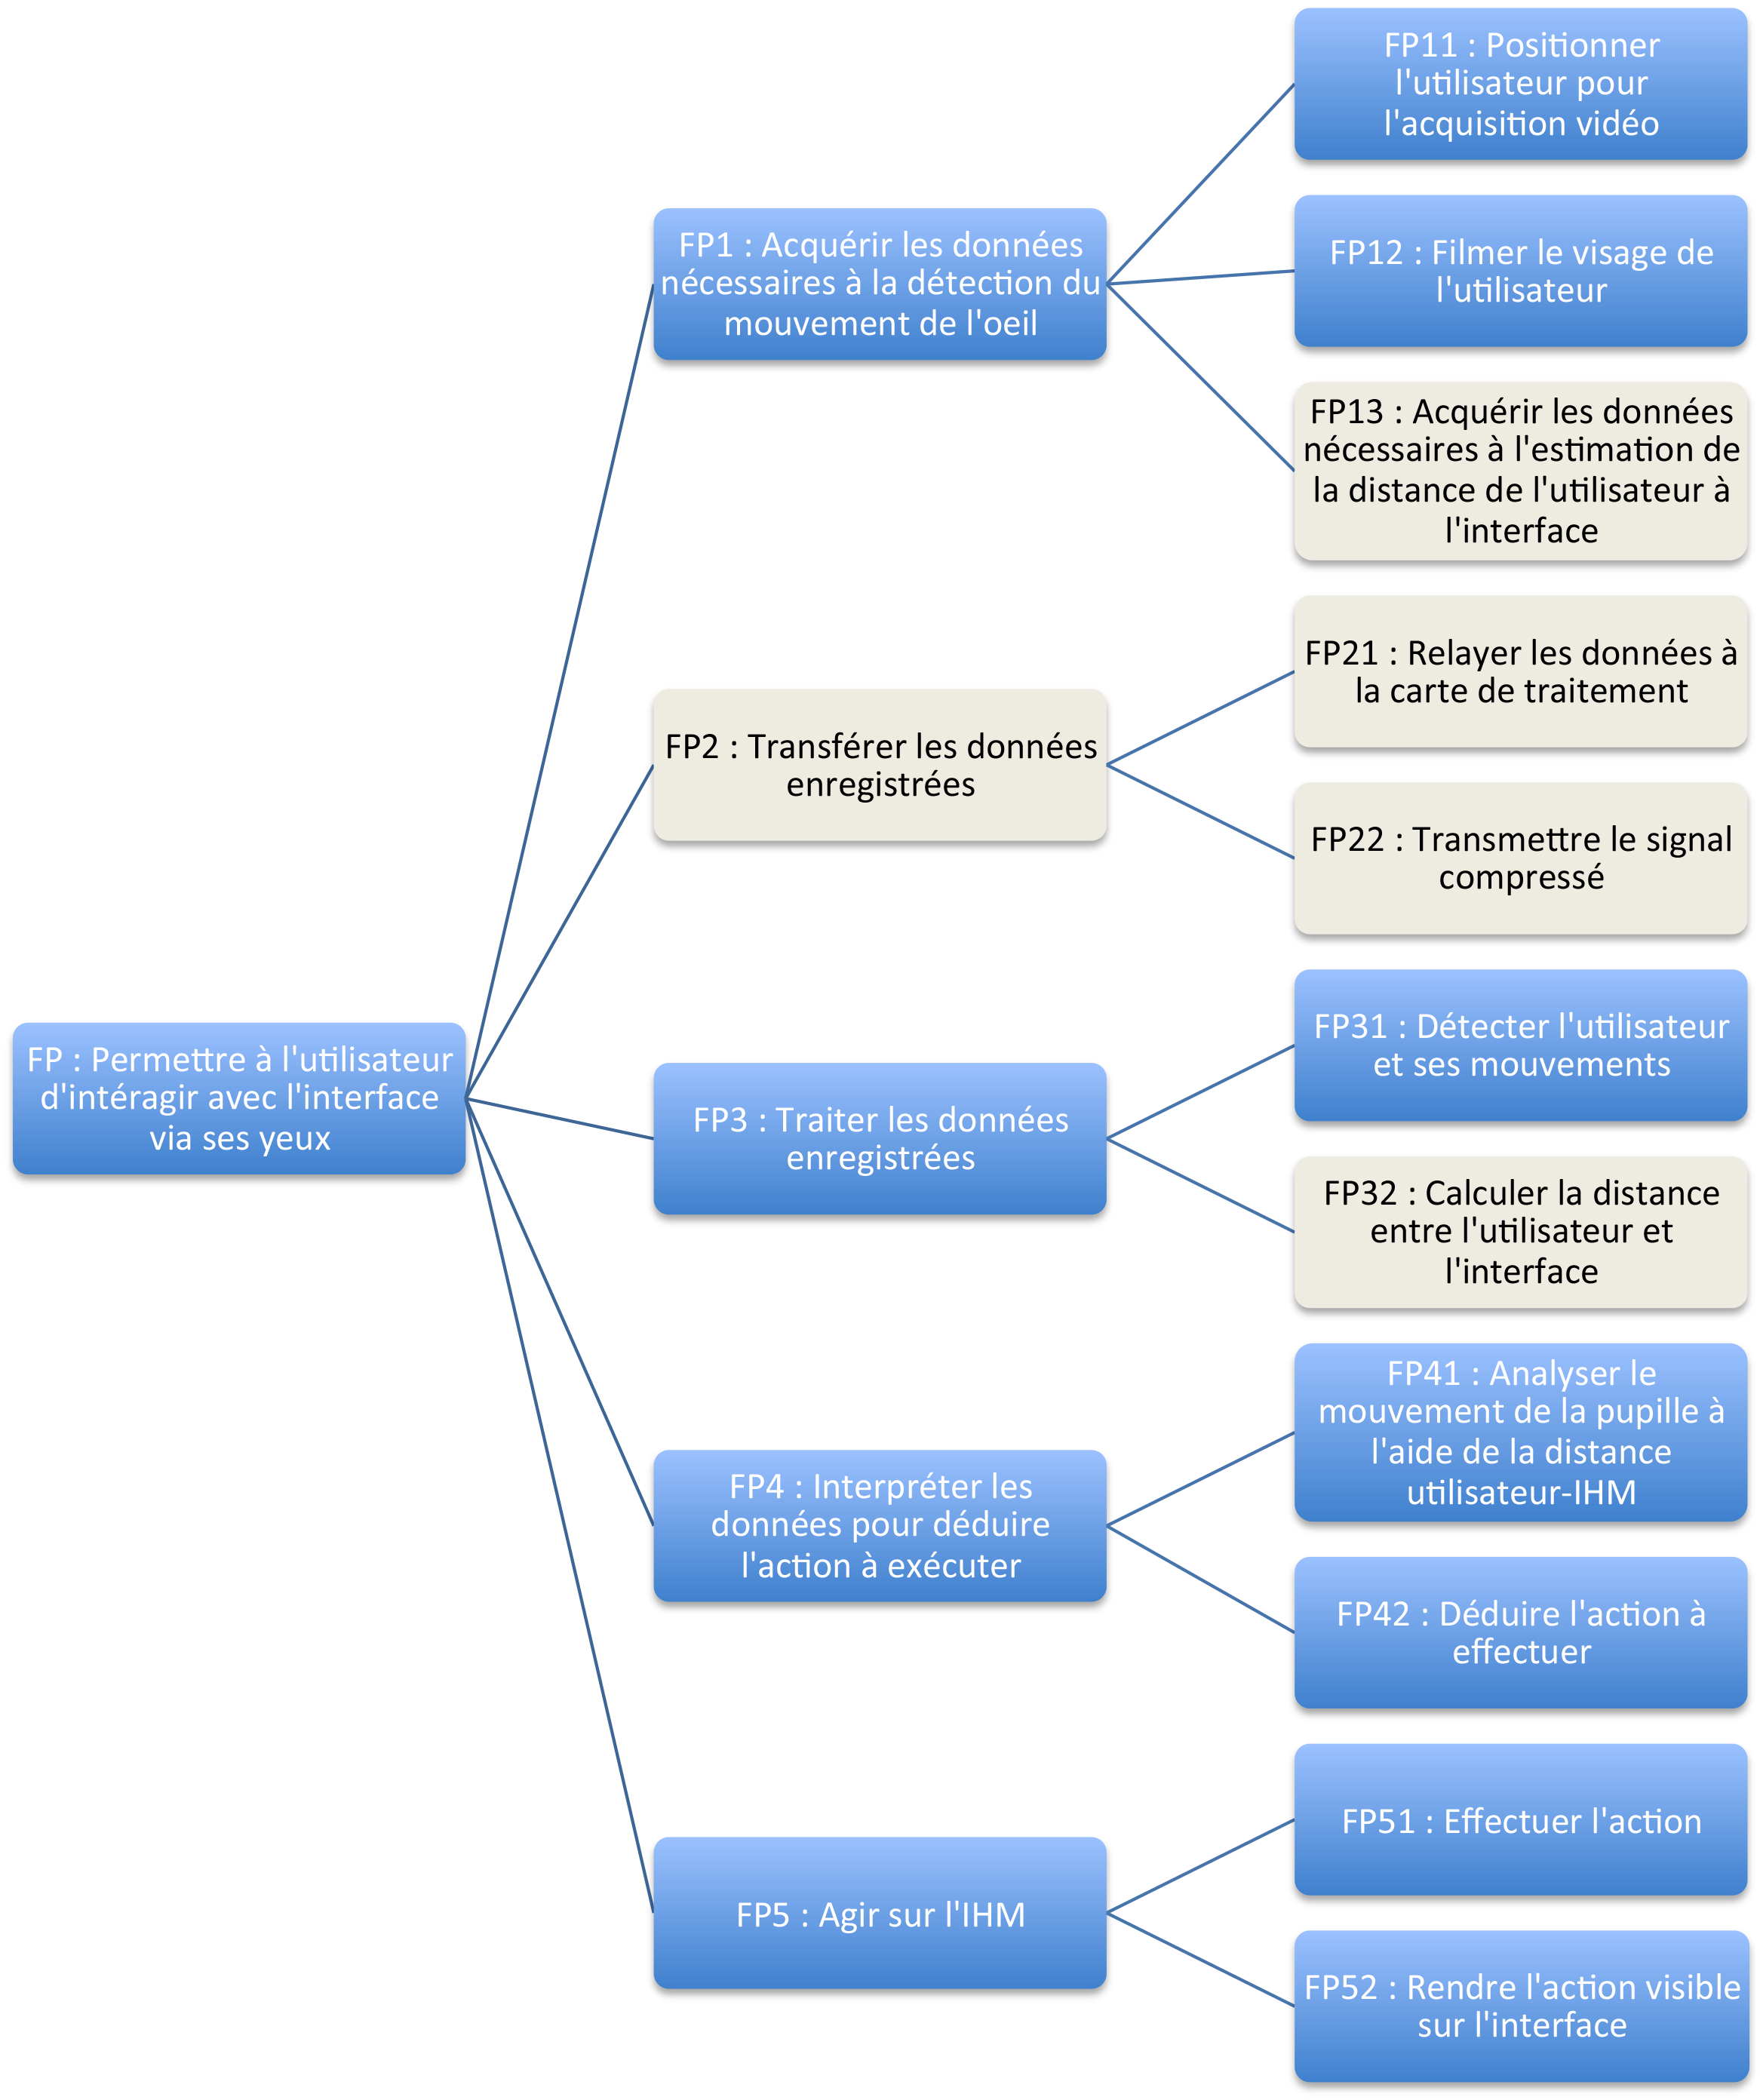
\includegraphics[scale=0.70]{FASTV2}
  \caption{FAST raffiné}
  \label{fig:FAST}
\end{figure}

Le cahier des exigences précédant nous a permis de définir les fonctions principales du système. Nous avons alors cherché à les raffiner par la méthode FAST (cf. figure \ref{fig:FAST}) pour obtenir des fonctions plus précises auxquelles nous pourrons apporter des solutions techniques propres à chacune. Nous pouvons ainsi entrevoir l'architecture fonctionnelle.

\subsection{Spécification des données}

La spécification du flux de données va permettre de comprendre les interactions et les échanges entre les différentes parties de notre système. Spécifier ainsi les données nous a permis de mieux comprendre les interactions entre chaque sous-partie du système. Il est ainsi clair que les données que nous allons principalement traiter et transférer seront des flux vidéos et qu’il sera donc important d’optimiser au mieux la rapidité de ces échanges.
Au travers de la figure \ref{fig:fluxDonnees}, nous pouvons aussi voir l’ordre avec lequel les sous-systèmes vont rentrer en jeu. Ainsi la Camera Narrow View sera dépendante du flux envoyé par la Camera Wide View. Un parallélisme de traitement des données est tout de même envisageable sur l'ordinateur pour gérer le flux vidéo de deux caméras.

\begin{figure}[h]
  \centering
  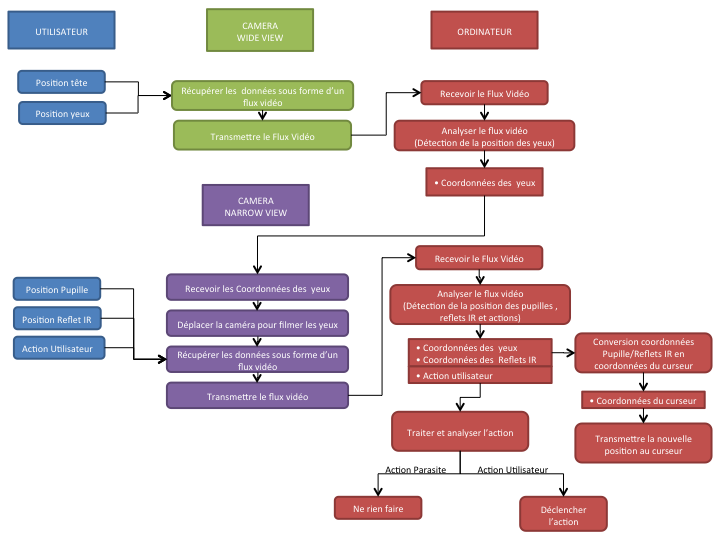
\includegraphics[scale=0.6]{FluxDonnees}
  \caption{Flux de données}
  \label{fig:fluxDonnees}
\end{figure}

\subsection{Spécification des comportements}

Le diagramme de séquence de la figure \ref{fig:comportementGlobal} illustre le comportement global du système. 

\begin{figure}[H]
  \centering
  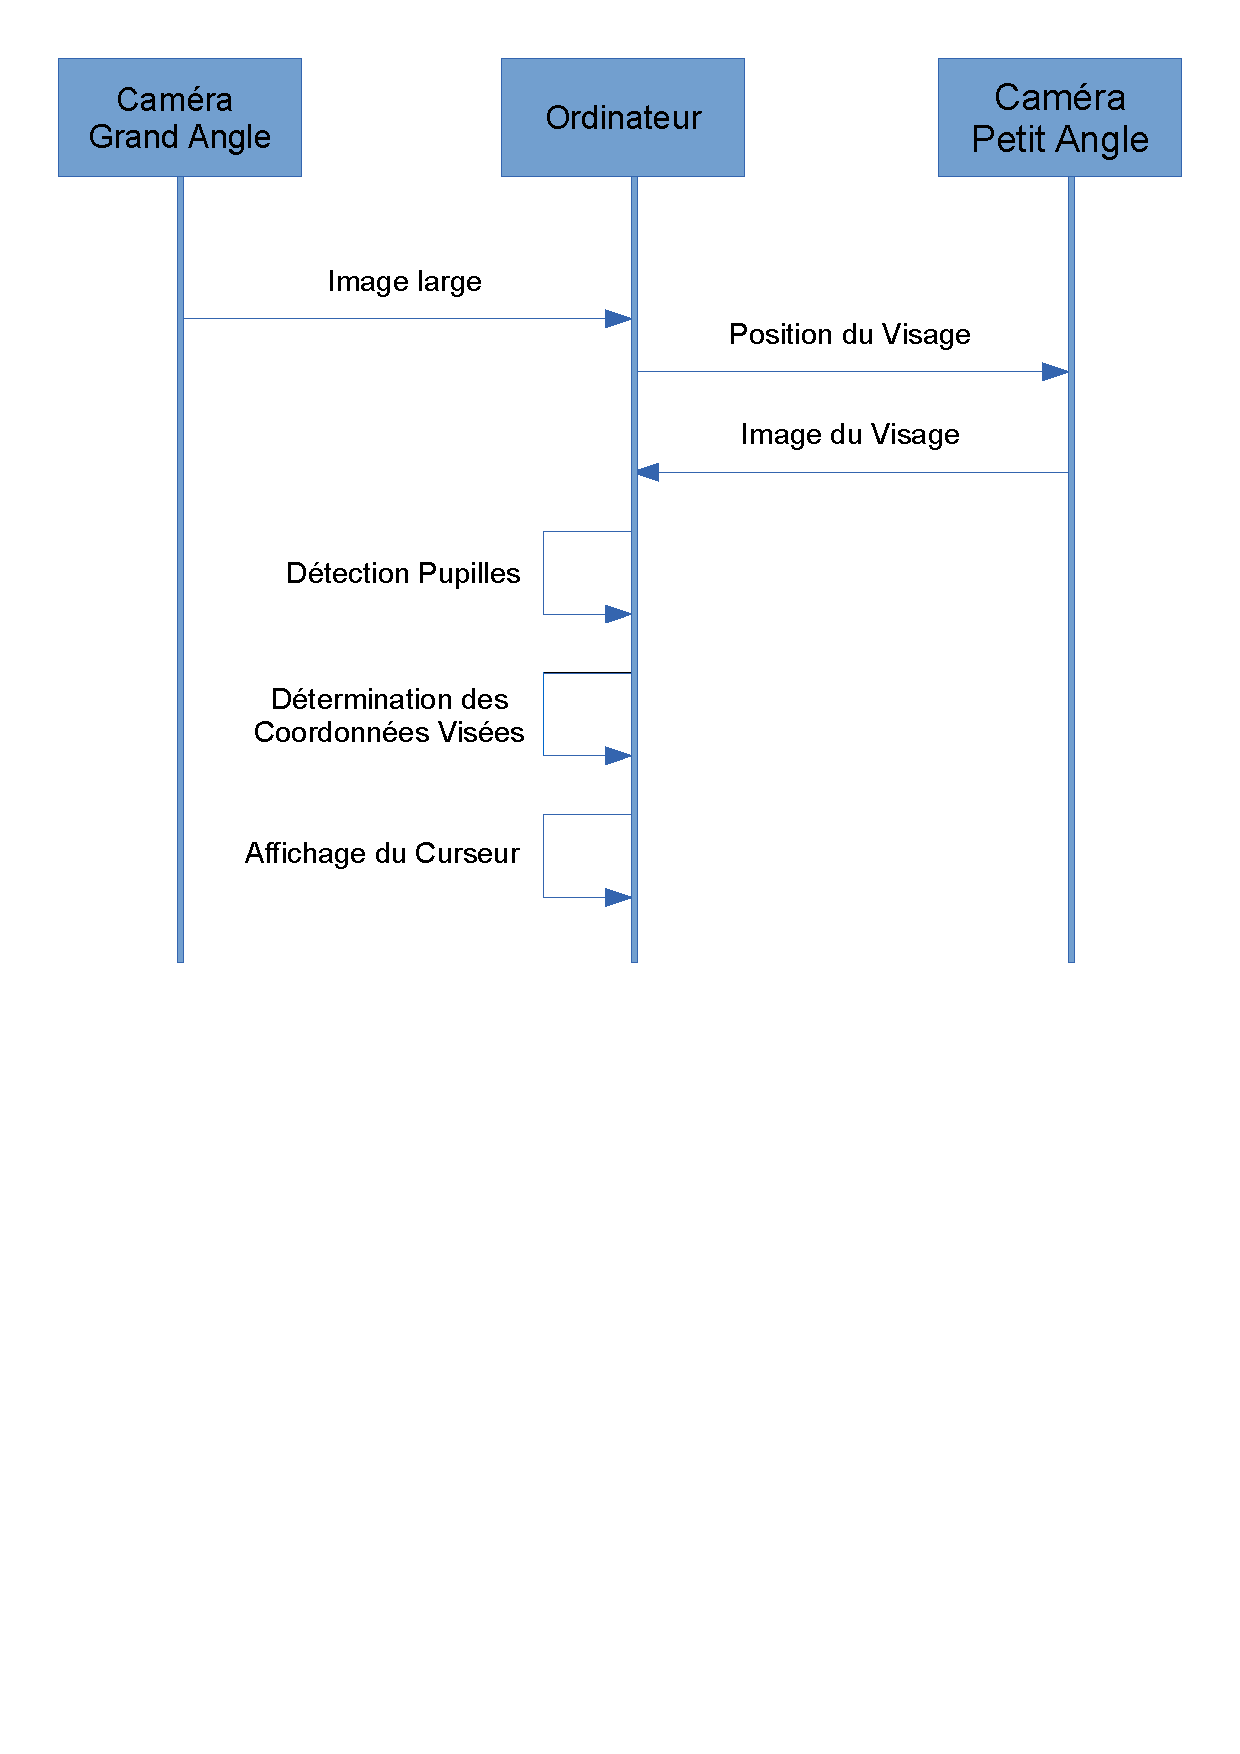
\includegraphics[scale=0.6]{comportementGlobal}
  \caption{Diagramme des spécifications du comportement global}
  \label{fig:comportementGlobal}
\end{figure}

\section{Architecture fonctionnelle}

Tout le travail réalisé au préalable sur la spécification fonctionnelle 3 axes permet finalement de proposer une architecture fonctionnelle pour notre système (cf. figure \ref{fig:archiFonctionnelle}).
 
\begin{figure}[H]
  \centering
  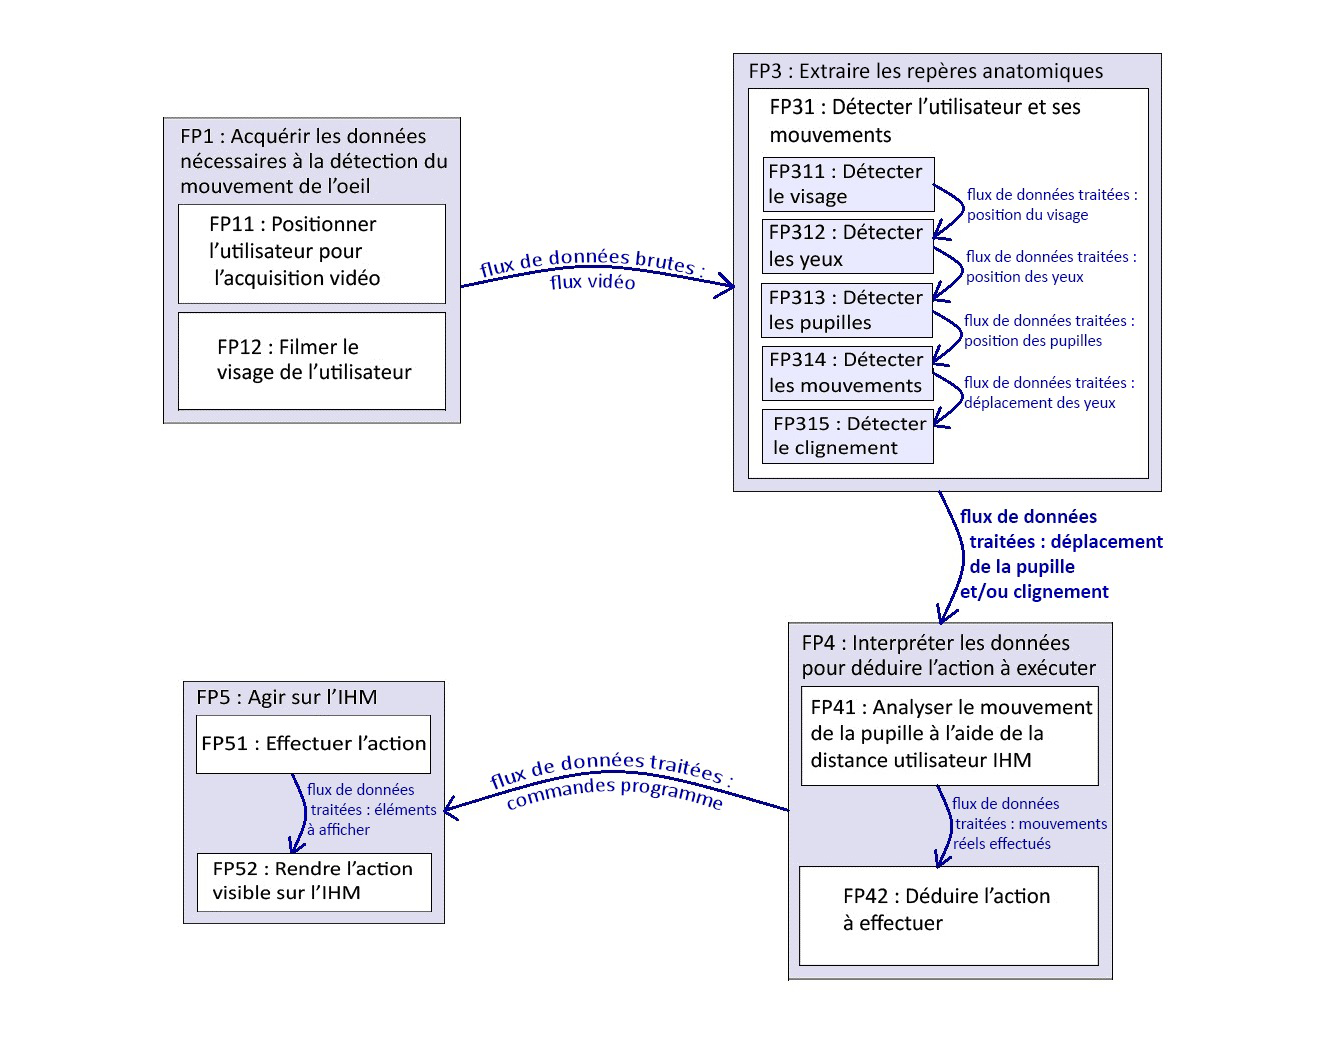
\includegraphics[scale=1.2]{ArchitectureFonctionnelle}
  \caption{Architecture Fonctionnelle}
  \label{fig:archiFonctionnelle}
\end{figure}

